\scanpage{40}
\unsure{10)|19)} (Modulo conjecture de Hodge) $G^{\circ}$ est engendré sur $\unsure{\mathbb Q|Q}$ par $i_1^{\mathbb C}$.

\deleted{\unsure{10)} $G$}

% slanted
\margin{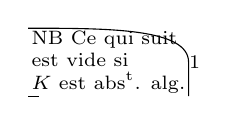
\begin{tikzpicture}[baseline=(current bounding box.north),font=\scriptsize]
\node[align=left,inner sep=1pt] (note) {\uline{NB} Ce qui suit\\est vide si\\$K$ est abs\textsuperscript{t}. alg.};
\draw (note.north west) .. controls (note.north) and (note.north east) .. (note.east)
.. controls (note.east) and (note.south east) .. (note.south east);
\draw (note.south west) -- ([xshift=4pt]note.south west);
\node[anchor=west,inner sep=0pt] at (note.east) {\deleted{\illegible{1}}};
\end{tikzpicture}}
Soit $R\subset G$ le sous groupe algébrique engendré par $w(\pi_1(S(\mathbb C),\xi))$. Il est \uline{invariant} moyennant \unsure{9)|4)} [car l'image fermée de $\pi_1(S(\mathbb C),\unsure{\xi|1})\relbar\pi_1(S,\xi)$\} est un sous-groupe invariant\}, le quotient étant $\pi_1(\operatorname{Spec} k,\xi)$, où $k$ est la clôture alg. de $\mathbb Q$ dans $K$]. \deleted{Le \unsure{composé}} En vertu de 4), l'hom.
\diagram{\begin{tikzcd}[ampersand replacement=\&,column sep=1.4em,row sep=.5ex]
{} \& {} \& \inserted{\widetilde G(\mathcal A),\ \text{où }\widetilde G=G/R,}\\
\pi_1(S\unsure{\mathbb C|\in},\xi) \arrow[r] \& G(\unsure{\mathcal A|\mathscr A|A}) \arrow[ur] \& {}
\end{tikzcd}}
se factorise donc en
\[
\tilde u:\underset{\substack{\Vert\\[-.4ex]\simeq\\[-.4ex]\unsure{\pi_1|\Vert}}}{\pi_1(\operatorname{Spec}(k),\xi)}
\longrightarrow\widetilde G(\mathcal A)
\]

D'autre part, on considère le torseur $\widetilde P=P/R$ sous $\widetilde G$, avec la connexion intégrable déduite de celle de $P$. On a

\margin{\deleted{\uline{\illegible{1}}}}
\unsure{16)|18)|10)} \inserted{(Modulo Hodge)} $(\widetilde P,\widetilde G)$ avec sa connexion intégrable ``se descend à $k$'', donc on a un torseur $(\widetilde P_0,(\widetilde G/k)$ sur $k$, et un isom de torseurs
\begingroup
\csname tagsleft@true\endcsname
\[
\widetilde P=P/R\simeq\widetilde P_0\otimes_k K \tag*{(*)}
\]
\endgroup

\deleted{De plus, \deleted{posant} introduisant $R'\subset G'$ correspondant à $R$, et $\widetilde G'=G'/R'$, de sorte qu'on a un isom}
\[
\deleted{\widetilde G'=\widetilde G'_0\otimes_k K,\qquad
\widetilde G'_0=\underline{\operatorname{Aut}}_{(\widetilde G/k)-}(\widetilde P_0),}
\]
\deleted{le ss-groupe \deleted{$\unsure{\widetilde H'|H'}\subset\unsure{\widetilde G'|G'}$} \inserted{$\widetilde H'=H'/H'\cap R'\unsure{=|\simeq}\operatorname{Im}(H'\longrightarrow\widetilde G')$} est ``défini sur $k$'' i.e. provient de $\widetilde H'_0\subset\widetilde G'_0$}

\inserted{Enfin l'isom \unsure{(*)|ci}, $\unsure{\in|\xi}$ qui} \deleted{La structure de filtration sur le foncteur $T$} définit, pour un $\widetilde G$-module $M$, une structure de descente sur $P\mathbin{\times}^{G_K}M_K$ à $k$\unsure{,|;} [c'est celle définie par la connexion intégrable de $P\mathbin{\alpha}^{G_K}M_K$], donne une donnée de descente \uline{compatible} avec la filtration, i.e cette dernière est \uline{horizontale}, $\bigl[\!\bigl[$ donc \deleted{\illegible{1}} $\widetilde H'=\operatorname{Im}(H'\longrightarrow\widetilde G')$, $\widetilde Q,=Q\mathbin{\times}^{\unsure{H'|\widetilde H'}}\widetilde H'$, se descendent \unsure{respect\textsuperscript{t}|respectiv\textsuperscript{t}} en $\widetilde H'_0\subset\widetilde G'$ et un torseur à droite $Q_0$ sous $\widetilde H'_0$, \unsure{\deleted{et}|et} (d'où $\widetilde H''_0$ et $\widetilde G''_0$ qui descendent $H''$ et $\widetilde G''$), et \deleted{\unsure{après}} les composés $\tilde i_1,\tilde i_2:\mathbb G_m\underset K{\relbar}G''\longrightarrow\widetilde G''$ se descendent en $(\tilde i_1)_0,(\tilde i_2)_0:\mathbb G_{m\,k}\longrightarrow\widetilde G''_0$ $\bigr]\!\bigr]$.
% archive sheet number: 39
